\chapter{Planificación e custos}

\section{Desenvolvemento}
O desenvolvemento desta aplicación levouse a cabo en varios sprints ou iteracións Scrum, creando para cada un deles o Sprint backlog, é dicir, o conxunto de funcionalidades a implementar. Os casos de uso desenvolvidos fóronse incrementando, aumentando dese xeito o número de funcionalidades dispoñíbeis.

Cada una destas iteracións foi dividida en catro fases distintas que se identifican coa planificación clásica dun proxecto: análise, deseño, implementación e probas.

No inicio do desenvolvemento decidiuse que a duración de cada sprint sería de 30 días.

Antes de comezar o primeiro sprint adicouse tempo á formación na programación para Android, así coma no uso de Android Studio e a realización de probas nun terminal físico e emulado pois era a primeira vez que se utilizaban estas tecnoloxías.

\subsection{Sprint 1: Aplicación Android: localización dentro dun edificio}
O obxectivo desta primeira iteración é a creación dos elementos básicos para a utilización dos sistemas de localización en interiores de Situm, permitindo aos usuarios ter un primeiro achegamento a esta tecnoloxía. Nesta primeira iteración só precisaremos construír unha aplicación para Android, deixando funcionalidades que requiran máis infraestrutura para seguintes sprints.

Para este sprint non se implementará a selección de contas de Situm nin a autenticación, polo que o rol dos usuarios que a utilicen será de Usuario Android anónimo cunha conta de Situm fixa. Só existirá unha actividade cun fragmento onde se mostrará o mapa.

A continuación veremos unha lista cos casos de uso implementados nesta iteración:

\begin{itemize}
	\item Visualizar o mapa dun edificio. Ver caso de uso \ref{tab:cuAmosarMapaEdificio}.
	\item Localizar un usuario dentro dun edificio. Ver caso de uso \ref{tab:cuLocalizacion}.
	\item Cambiar de piso dentro dun edificio. Ver caso de uso \ref{tab:cuCambiarPiso}.
\end{itemize}

\paragraph{Fito}
Ao final deste sprint teremos unha aplicación simple pero funcional, na que se poderá localizar usuarios dentro de edificios configurados para a súa utilización con Situm. Permitirá ao cliente observar as posibilidades de localización de Situm dentro dun edificio e comprobará a súa exactitude.

\paragraph{Proba}
A proba para validar as tarefas implementadas será a utilización da aplicación dentro dun edificio con varios niveis, movéndose en toda a súa extensión. Desta maneira observaranse as posibilidades de localización da nosa plataforma e o bo funcionamento do cambio de niveis, tanto fisicamente como seleccionándoo no mapa.


\subsection{Sprint 2: Servidor inicial: POIs e percorridos}
O obxectivo desta segunda iteración é a creación das funcións básicas do servidor e o seu despregue para poder ser utilizado nun entorno de produción. Neste punto aínda non se traballará na integración coa aplicación Android senón que nos centraremos unicamente no servidor.

Traballarase na arquitectura xeral do servidor e nas súas diferentes capas, polo que ao final deste sprint teremos uns servizos web ampliábeis de xeito doado. Crearanse servizos para a recuperación de información sobre os puntos de interese e os percorridos almacenados nunha base de datos.

O administrador do sistema será o encargado de inserir a través dun programa xestor os datos recuperados pola aplicación. Estes datos serán novos edificios, puntos de interese e percorridos.

A continuación veremos os casos de uso da parte servidora nos que se traballou neste sprint:

\begin{itemize}
	\item Dar de alta edificio. Ver caso de uso \ref{tab:cuAltaEdificio}.
	\item Amosar lista de POIs. Ver caso de uso \ref{tab:cuAmosarListaPOI}.
	\item Amosar información dun POI. Ver caso de uso \ref{tab:cuAmosarPOI}.
	\item Amosar lista de percorridos. Ver caso de uso \ref{tab:cuAmosarListaPercorrido}.
	\item Amosar información dun percorridos. Ver caso de uso \ref{tab:cuAmosarPercorrido}.
\end{itemize}

\paragraph{Fito}
Ao final deste sprint obteremos un servidor utilizábel dende calquera lugar e cuns casos de uso básicos para comprobar o seu funcionamento.

\paragraph{Proba}
As probas realizadas serán levadas a cabo nun entorno local e noutro de produción, co despregue do servidor a través dos servizos de Amazon (AWS). Realizaranse chamadas para recuperar a información a través dos servizos publicados.

\subsection{Sprint 3: Lectura datos dende aplicación Android}
Na terceira iteración do noso proxecto búscase a ligazón entre a aplicación Android e o servidor, que ata este punto levaron camiños paralelos. Modificarase a aplicación Android para recibir a información fornecida polo servidor, procesaraa e mostraraa por pantalla. Neste sprint tampouco se traballará con outro rol que non sexa o de Usuario Android anónimo.

En canto aos casos de uso tratados nesta iteración, aparte de completar coa parte de vista os comezados no sprint anterior, implementáronse os seguintes:

\begin{itemize}
	\item Amosar POI no mapa. Ver caso de uso \ref{tab:cuAmosarPOIMapa}.
	\item Amosar percorrido no mapa. Ver caso de uso \ref{tab:cuAmosarPercorridoMapa}.
\end{itemize}

\paragraph{Fito}
Ao final deste sprint teremos por primeira vez unha visión xeral do que proporcionará a nosa plataforma, unindo a potencia de Situm cos nosos propios datos, permitindo amosar puntos de interese e percorridos. Poderase visualizar no mapa da aplicación os POIs e percorridos almacenados na nosa base de datos e acceder á súa información.

\paragraph{Proba}
A proba para validar as tarefas implementadas consistirá na utilización da aplicación nun edificio configurado en Situm con información sobre puntos de interese e percorridos no noso sistema.

\subsection{Sprint 4: Autenticación de usuarios}
Neste sprint tratarase a autenticación dos usuarios a través dos servizos de Google \cite{googleSignIn}. Almacenaremos estes usuarios autenticados para establecer permisos nos distintos edificios. Tamén se permitirá a selección de contas de Situm, polo que debemos proporcionar unha lista coas contas dispoñíbeis sexan públicas ou estean asociadas ao usuario autenticado.

A continuación veremos unha relación cos casos de uso nos que se traballou neste sprint:

\begin{itemize}
	\item Autenticarse a través de Google. Ver caso de uso \ref{tab:cuAutenticar}.
	\item Facer logout. Ver caso de uso \ref{tab:cuLogout}.
	\item Dar de alta unha conta de Situm. Ver caso de uso \ref{tab:cuDarAltaContaSitum}.
	\item Recuperar as contas de Situm dispoñíbeis. Ver caso de uso \ref{tab:cuRecuperarContasSitum}.
\end{itemize}

\paragraph{Fito}
Ao final deste sprint teremos unha actividade inicial onde o usuario poderá autenticarse a través dunha conta de Google para acceder á aplicación. Esta autenticación tamén lle proporcionará a posibilidade de ter acceso a máis contas de Situm, o que provocará que poida ver novos edificios asociados a esas contas.

\paragraph{Proba}
A proba para validas este sprint consistirá na utilización da aplicación con varias contas de Google que teñan distintos permisos sobre contas de Situm, para comprobar desta maneira que non están todas dispoñíbeis para usuarios anónimos ou con distintas contas de Google.

\subsection{Sprint 5: Edición de POIs e percorridos dende a aplicación Android}
Ata este sprint a creación dos datos para a nosa aplicación tiña que ser directamente sobre a base de datos cun xestor. Neste sprint cubriranse os casos de uso que permitan realizar estas modificacións directamente dende a aplicación Android, incorrendo nun menor esforzo. Neste sprint fai a súa aparición o rol Xestor de contido, que será o encargado da xestión dos puntos de interese e percorridos.

A continuación veremos unha relación cos casos de uso nos que se traballou neste sprint:

\begin{itemize}
	\item Xestión de POIs: Creación. Ver caso de uso \ref{tab:cuCrearPOI}.
	\item Xestión de POIs: Modificación. Ver caso de uso \ref{tab:cuModificarPOI}.
	\item Xestión de POIs: Borrado. Ver caso de uso \ref{tab:cuEliminarPOI}.
	\item Xestión de percorridos: Creación. Ver caso de uso \ref{tab:cuCrearPercorrido}.
	\item Xestión de percorridos: Modificación. Ver caso de uso \ref{tab:cuModificarPercorrido}.
	\item Xestión de percorridos: Borrado. Ver caso de uso \ref{tab:cuEliminarPercorrido}.
	\item Engadir POI a percorrido. Ver caso de uso \ref{tab:cuEngadirPOIPercorrido}.
	\item Eliminar POI de percorrido. Ver caso de uso \ref{tab:cuEliminarPOIPercorrido}.
	\item Dar permisos a usuario sobre un edificio. Ver caso de uso \ref{tab:cuDarPermisoUsuarioEdificio}.
\end{itemize}

\paragraph{Fito}
Ao final deste sprint teremos unha aplicación completamente funcional, coa posibilidade da edición dentro da mesma sen ter que recorrer a elementos externos.

\paragraph{Proba}
O primeiro paso para as probas deste sprint consistirá na creación, modificación e borrado de POIs ao longo dun edificio, en distintas plantas e con diferentes usuarios. Posteriormente utilizaremos eses puntos de interese para a creación de diversos percorridos, que tamén serán editados (tanto a súa información coma a inserción de POIs despois de ter creado o percorrido) e borrados. Tamén se deberá comprobar as opcións dispoñíbeis para os usuarios en base aos roles asignados.


\subsection{Sprint 6: Valor engadido da localización Situm}
O obxectivo do sexto sprint é a utilización da localización en Situm para proporcionarlle máis servizos ao usuario. Non se precisará ningún permiso especial para utilizar esta capacidade, que permitirá guiar aos usuarios a un punto de interese ou seguir todo un percorrido. A ruta de guiado será actualizada automaticamente pola aplicación mentres o usuario non o cancele. Tamén se lle permitirá aos xestores de contido estimar o tempo adicado a cada POI e percorrido.

A continuación veremos unha relación cos casos de uso nos que se traballou neste sprint:

\begin{itemize}
	\item Guiar ata un punto de interese. Ver caso de uso \ref{tab:cuGuiarPOI}.
	\item Guiar a través dun percorrido. Ver caso de uso \ref{tab:cuGuiarPercorrido}.
	\item Estimar tempo adicado a POI. Ver caso de uso \ref{tab:cuEstimarTempoPOI}.
	\item Estimar tempo adicado a percorrido. Ver caso de uso \ref{tab:cuEstimarTempoPercorrido}.
\end{itemize} 

\paragraph{Fito}
Ao final deste sprint o usuario poderá ser guiado aos puntos de interese do edificio, así como poder utilizar esta capacidade en edificios, sabendo canto tempo estimado lle levará cada visita grazas aos novos valores de cada POI e percorrido.

\paragraph{Proba}
As probas para validar este sprint consistirán no guiado dentro dun edificio configurado a través de Situm mediante as rutas creadas no seu dashboard.

\subsection{Sprint 7: Imaxes para POIs}
O obxectivo do sétimo sprint é a xestión de imaxes para os puntos de interese. Os xestores de contido poderán engadir as imaxes que consideren oportunas a calquera POI dentro dun edificio para que visualicen os usuarios da aplicación. Non se precisará ningún permiso a maiores, chega con ser xestor de contido dun edificio. Non haberá límite de imaxes para os puntos.

A continuación veremos unha relación cos casos de uso nos que se traballou neste sprint:

\begin{itemize}
	\item Amosar lista de imaxes dun POI. Ver caso de uso \ref{tab:cuCrearPOI}.
	\item Amosar imaxe dun POI. Ver caso de uso \ref{tab:cuModificarPOI}.
	\item Xestión de imaxes: Engadir. Ver caso de uso \ref{tab:cuCrearPercorrido}.
	\item Xestión de imaxes: Modificar datos. Ver caso de uso \ref{tab:cuModificarPercorrido}.
	\item Xestión de imaxes: Eliminar. Ver caso de uso \ref{tab:cuEliminarPercorrido}.
\end{itemize} 

\paragraph{Fito}
Ao final deste sprint teremos a opción de administrar imaxes sobre os puntos de interese e visualizalas para permitir dar maior información sobre cada un deles.

\paragraph{Proba}
As probas para validar este sprint consistirán no engadido e eliminación de imaxes dentro dos POIs dun edificio por parte dun xestor de contido. Débese comprobar que a un usuario Android normal non se lle permita o engadido ou eliminación de imaxes. Ambos roles (xestor de contido e usuario Android) deben poder ver as imaxes dos POIs.


\section{Planificación e custos iniciais}
A continuación pódense observar tanto a planificación inicial do proxecto coma os custos asociados a esta. No terceiro punto descríbense os plans de continxencia preparados para o proxecto.

\subsection{Planificación inicial}
Nesta sección describirase a planificación completa e detallada do proxecto. O primeiro paso para realizala foi establecer o alcance do proxecto e os requisitos precisos para poder levalo a cabo. Na primeira planificación fíxose un bosquexo xeral dos pasos a seguir no proxecto, estimando unha duración do desenvolvemento contando con sete sprints dunhas tres semanas cada un. Debido ao horario dispoñíbel polo traballador, considerouse unha xornada laboral de catro horas diarias.

Pódese observar o diagrama de Gantt coa planificación detallada na figura~\ref{fig:planificacionInicial}. Diferéncianse todos os pasos realizados no proxecto, así como o tempo adicado a cada sprint.

\begin{figure}[tbh] 
	\begin{center}
		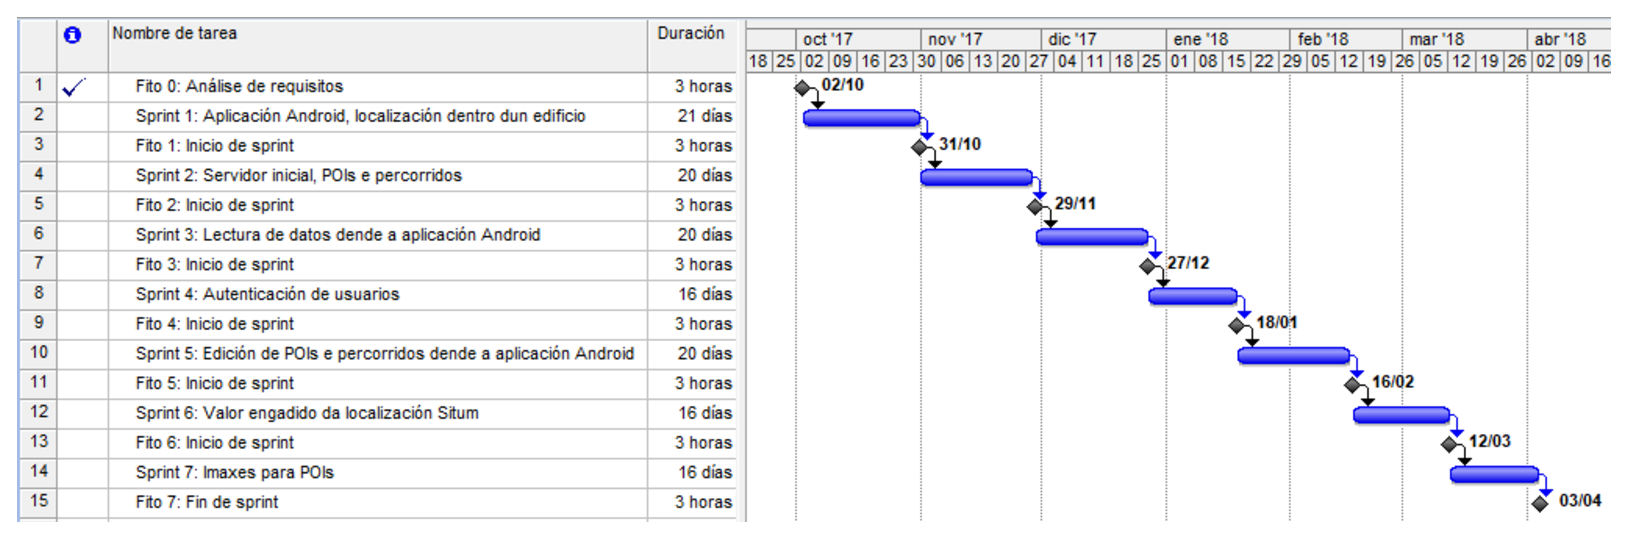
\includegraphics[width=1\textwidth]{figures/Capturas/planificacionInicial}
		\caption{Diagrama de Gantt da planificación inicial para os sprints.}
		\label{fig:planificacionInicial}
	\end{center}
\end{figure}

\subsection{Custo inicial}
Unha vez realizada a planificación das tarefas nas que se divide o proxecto pódese comezar coa análise económica dos custos asociados. Como é evidente, o custo máis alto recae sobre os recursos humanos, xa que os materiais utilizados non demandaron moita inversión.

\paragraph{Recursos humanos}
Ao ser un proxecto elaborado por un único traballador, tivo que realizar varias funcións que normalmente recaerían sobre distintas persoas, polo que asignamos distintos valores ao seu traballo dependendo da función que realizase en cada momento. Considérase xefe de proxecto ao titor do proxecto que realiza tarefas de supervisión e exerce de scrum master nas xuntanzas entre sprints.
O tempo estimado para o xefe de proxecto coincide cos fitos de inicio e fin de sprint, polo que terá que actuar 8 veces.
Na táboa ~\ref{tab:horasTraballo} pódese observar a descomposición da estimación inicial por tarefa para o analista e o programador.

\begin{table} [tbh]
	\footnotesize
	\centering
	\begin{tabular}{|l|c|c|}
		\hline 
		\textbf{Sprint} & \textbf{Analista} & \textbf{Programador} \\ 
		\hline 
		Primeiro & 14 h & 70 h \\ 
		\hline 
		Segundo & 11 h & 69 h \\ 
		\hline 
		Terceiro & 13 h & 67 h \\ 
		\hline 
		Cuarto & 10 h & 54 h \\ 
		\hline 
		Quinto & 13 h & 67 h \\ 
		\hline 
		Sexto & 10 h & 54 h \\ 
		\hline 
		Sétimo & 10 h & 54 h \\ 
		\hline 
	\end{tabular}
	\caption{Horas planificadas para o traballador.}
	\label{tab:horasTraballo}
\end{table}

Pódense observar os custos asociados aos recursos na táboa~\ref{tab:custoPersoalInicial}.

\begin{table} [tbh]
	\footnotesize
	\centering
	\begin{tabular}{|l|c|c|c|}
		\hline 
		\textbf{Recurso} & \textbf{Salario (€/h)} & \textbf{Tempo (h)} & \textbf{Custo} \\ 
		\hline 
		Xefe de proxecto & 50 & 24 & 1.200 € \\ 
		\hline 
		Analista & 37 & 81 & 2.997 € \\ 
		\hline 
		Programador & 20 & 516 & 10.320 € \\ 
		\hline 
		Formación & 0 & 40 & 0 € \\ 
		\hline 
		\multicolumn{3}{ |l| }{Total} & 14.517 € \\ 
		\hline 
	\end{tabular}
	\caption{Custos planificados en recursos humanos.}
	\label{tab:custoPersoalInicial}
\end{table}

\paragraph{Recursos materiais}
Podemos dividir os recursos materiais en hardware e software. Non houbo gastos referidos ao software posto que se utilizou software gratuíto na realización do proxecto, mais si que houbo gastos en canto aos recursos hardware. Houbo que realizar un desembolso polo ordenador utilizado para a programación do proxecto posto que a emulación dun terminal Android é bastante custosa e unha computadora antiga non era capaz de executalo. Tamén se inclúen nos gastos un móbil de gama media para a proba da aplicación en entornos reais. Mención aparte require a subscrición a Amazon Web Services, posto que se desfrutou dun período de proba que, non obstante, non estaría dispoñíbel unha vez a aplicación requira un maior uso de recursos por parte do servidor. Este tipo de servizos supoñen un maior custo canta máis demanda procesan, polo que en entornos reais de produción o custo aumentaría.
Os gastos debido aos recursos materiais pódense ver na táboa~\ref{tab:custoMaterial}. Non imputamos ao proxecto o custo do PC de sobremesa nin do teléfono móbil pois ambos foron utilizados para outros usos á marxe do proxecto e polo tanto, amortizados.

\begin{table} [tbh]
	\footnotesize
	\centering
	\begin{tabular}{|l|c|c|}
		\hline 
		\textbf{Recurso} & \textbf{Custo} & \textbf{Imputado ao proxecto} \\ 
		\hline 
		PC sobremesa & 860 € & 0 € \\ 
		\hline 
		Teléfono móbil & 440 € & 0 € \\ 
		\hline 
		\multicolumn{2}{ |l| }{Total} & 0 € \\ 
		\hline 
	\end{tabular}
	\caption{Custos en recursos materiais.}
	\label{tab:custoMaterial}
\end{table}


\paragraph{Total}
Despois de analizar os custos en recursos humanos e materiais podemos establecer o custo total inicial. Obsérvanse todas as entradas na táboa~\ref{tab:custoTotalEstimado}:

\begin{table} [tbh]
	\footnotesize
	\centering
	\begin{tabular}{|l|c|}
		\hline 
		\textbf{Tipo de recurso} & \textbf{Custo} \\ 
		\hline 
		Recursos humanos & 14.517 € \\ 
		\hline 
		Recursos materiais & 0 € \\ 
		\hline 
		Total & 14.517 € \\ 
		\hline 
	\end{tabular}
	\caption{Custos totais estimados.}
	\label{tab:custoTotalEstimado}
\end{table}

\subsection{Análise de riscos e plans de continxencia}
Neste punto trátase a análise de todos os riscos máis importantes que se poden producir na elaboración do proxecto xunto coa posibilidade de que se produzan, para despois elaborar plans de continxencia para cada un deles no caso de que afectasen ao traballo.

\paragraph{Riscos}
Na táboa~\ref{tab:riscos} pódense ver os riscos propios do proxecto realizado. Tivéronse en conta tanto a probabilidade de que se producisen estes erros (alta, media, baixa) coma o impacto sobre o desenvolvemento (alto, medio, baixo) para calcular a exposición ao risco (alta, media, baixa) e dese xeito poder ordenalos para atacar aqueles cunha maior exposición.
A continuación enumeramos os riscos detectados ao inicio do proxecto:

\begin{table} [tbh]
	\footnotesize
	\centering
	\begin{tabular}{|l|c|c|c|}
		\hline 
		\textbf{Risco} & \textbf{Probabilidade} & \textbf{Impacto} & \textbf{Exposición} \\ 
		\hline 
		Programación en Android & Alta & Baixo & Baixa \\ 
		\hline 
		Ferramentas descoñecidas & Alta & Baixo & Baixa \\ 
		\hline 
		Modificación de requisitos & Alta & Medio & Alta \\ 
		\hline 
		Interface de usuario non clara & Media & Medio & Media \\ 
		\hline 
		Dispoñibilidade do equipo & Media & Alta & Alta \\ 
		\hline 
	\end{tabular}
	\caption{Avaliación dos riscos do proxecto.}
	\label{tab:riscos}
\end{table}

\begin{itemize}
	\item Programación en Android: Debido a que o equipo de desenvolvemento nunca programara ningunha aplicación para Android, había un risco importante de retraso nos primeiros sprints.
	\item Ferramentas descoñecidas: Ao igual que o punto anterior, o equipo de desenvolvemento non tiña experiencia en programación coa SDK de Situm, nin con Google Maps.
	\item Modificación de requisitos: Ao ser un proxecto con tecnoloxía novedosa e en constante actualización é complicado definir claramente e con tempo as especificacións desexadas.
	\item Interface de usuario non clara: En relación co primeiro punto tratado, ao ser a primeira vez que o equipo realiza unha aplicación móbil, resulta moi probábel que a interface creada para a aplicación non sexa o suficientemente clara e atractiva por falta de experiencia real.
	\item Dispoñibilidade do equipo de desenvolvemento: O equipo de desenvolvemento está constituído por un único membro cun traballo a xornada completa, polo que a súa dispoñibilidade non será a desexada durante a duración do proxecto.
\end{itemize}

\paragraph{Plans de continxencia}
Débese ter especial coidado cos riscos cunha alta exposición, polo que se serán os que máis atención reciban:

\begin{itemize}
	\item Modificación de requisitos: Para evitar este risco a mellor maneira é a comunicación continua co cliente, polo que se deben ter xuntanzas periódicas co mesmo. Un dos puntos fortes da metodoloxía Scrum é precisamente a protección contra os cambios de requisitos.
	\item Dispoñibilidade do equipo de desenvolvemento: Ante a imposibilidade de realizar o traballo en horario laboral, deberase reservar as fins de semana para tratar de ter un calendario estábel para a creación do proxecto. Ao final de cada sprint realizarase un seguimento do esforzo realizado e formularase unha replanificación sempre que se considere necesario.
	\item Interface de usuario non clara: Buscarase unha selección de iconas o suficientemente representativas das accións dispoñíbeis na aplicación que permitan unha aproximación sinxela aos usuarios. Ao finalizar os sprints é recomendábel amosar as interfaces a posíbeis usuarios.
	\item Programación en Android: Os primeiros sprints deben ser o suficientemente folgados para unha aprendizaxe correcta das características propias da programación en Android.
	\item Ferramentas descoñecidas: Ao igual que ocorría no punto anterior, hai que ter en conta a programación coa SDK de Situm así coma dos métodos propios de Google Maps para que non provoquen un retraso importante.
\end{itemize}

\section{Planificación e custos finais}
Unha vez finalizado o proxecto pódese analizar a planificación final, con todas as incidencias producidas; así coma visualizar os custos reais e totais derivados do desenvolvemento.


\subsection{Planificación final}
Despois da realización do proxecto e superados todos os problemas xurdidos durante a súa elaboración, pásase a detallar a planificación final. Pódese observar o diagrama de Gantt final detallado na figura~\ref{fig:planificacionFinal}. En total, aumentouse o tempo de proxecto en 11 días laborais.
Unha vez finalizado o sétimo e último sprint do desenvolvemento, procedeuse á realización da memoria que levou tres semanas máis de traballo grazas a que durante as iteracións foise cubrindo parte da documentación. Estas últimas semanas débense á creación de parte dos apéndices así como as seccións de planificación, probas e conclusións.

\begin{figure}[tbh] 
	\begin{center}
		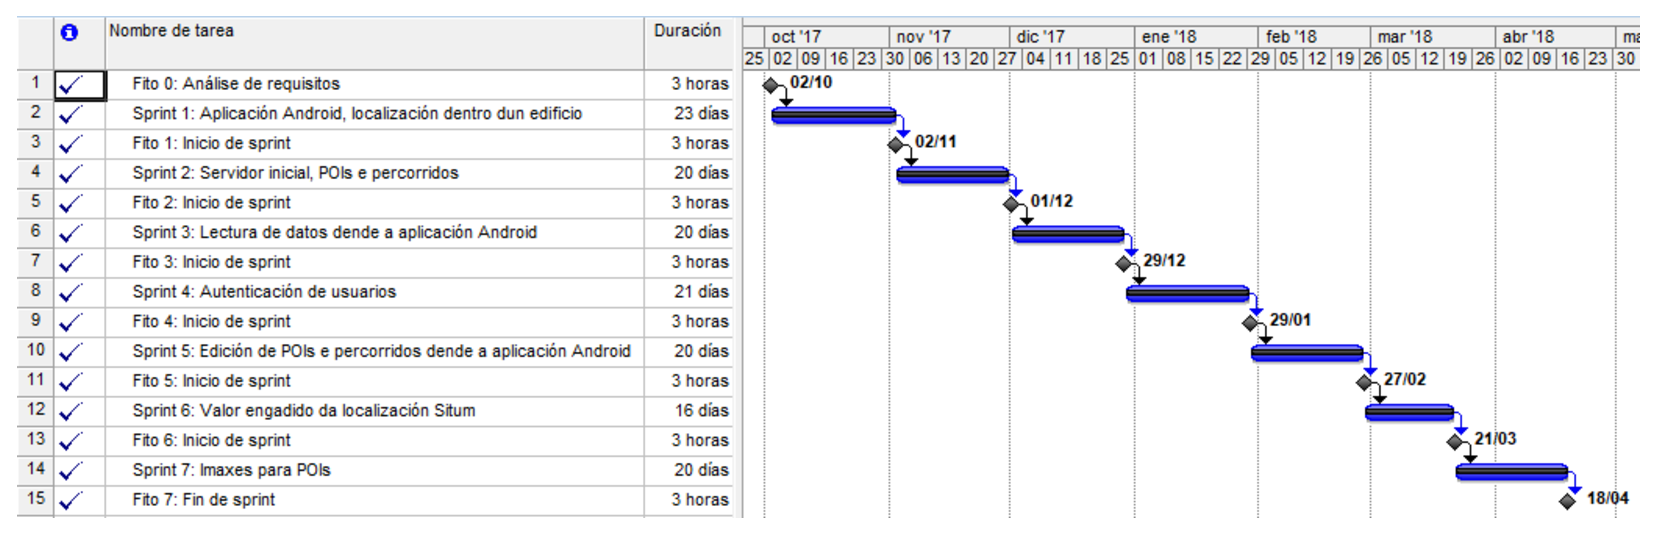
\includegraphics[width=1\textwidth]{figures/Capturas/planificacionFinal}
		\caption{Diagrama de Gantt para os sprints despois de realizar o seguemento ao proxecto.}
		\label{fig:planificacionFinal}
	\end{center}
\end{figure}

\subsection{Incidencias e resolución}
A continuación expóñense os problemas ocorridos durante o proxecto a como se resolveron, divididos por sprints:

\begin{itemize}
	\item Sprint 1: A pesar de telo presente na planificación, houbo que incrementar levemente o tempo adicado a esta iteración por mor da pouca destreza do programador nun entorno novo para el como é Android e tamén pola integración da aplicación con Google Maps. A representación dos mapas de interiores proporcionados por Situm foi outro dos puntos que afectou negativamente á planificación, mentres que o tratamento da posición e a posta en marcha da SDK de Situm foi bastante sinxela polo que contrarrestou o efecto da visualización dos mapas.
	\item Sprint 2: Esta iteración levouse a cabo no tempo estimado posto que o programador xa estaba afeito a este tipo de traballo.
	\item Sprint 3: A pesar do crítico deste paso, non se rexistrou unha demora na súa realización.
	\item Sprint 4: Con esta iteración non houbo ningún problema ata o momento de publicar a aplicación na tenda de Google Play \cite{googlePlayStore}, xa que houbo que reconfigurar Google Play Services por culpa do cifrado da aplicación. Non foi ata esta reconfiguración cando se puido realizar correctamente unha autenticación na aplicación descargada dende Google Play. Ao inicio descoñecíase o motivo polo cal non se permitía esta acción, o que provocou un aumento considerábel da duración do sprint.
	\item Sprint 5: A pesar de ser a iteración con máis contido dentro da planificación, non supuxo un problema a súa implementación posto que xa se avanzara o suficiente no proxecto como para estar cómodo no novo entorno e os casos de uso realizados non eran especialmente complexos.
	\item Sprint 6: Non houbo problemas inesperados nesta iteración.
	\item Sprint 7: O envío e recepción de imaxes a través do dispositivo móbil foi máis problemático do inicialmente esperado. A parte do servidor foi segundo o estimado xa que se puido validar a través da ferramenta Postman mais non así a integración coa aplicación móbil.
\end{itemize}

\subsection{Custo final}
Unha vez finalizado o proxecto, débese calcular o custo final. A única variación co custo calculado ao inicio recae sobre os recursos humanos, xa que non houbo ningún tipo de variación de prezo nos recursos hardware ou software, polo que soamente se tratará a variación por culpa dos retrasos nos sprints.

\paragraph{Recursos humanos}
A continuación indicaranse as horas de aumento con respecto á planificación tanto para o analista como para o programador. Os sprints que sufriron retrasos foron o primeiro, o cuarto e o sétimo. Na táboa~\ref{tab:horasTraballoReais} pódense ver as horas concretas.

\begin{table} [tbh]
	\footnotesize
	\centering
	\begin{tabular}{|l|c|c|c|c|}
		\hline 
		\textbf{Sprint} & \textbf{Analista} & \textbf{Variación analista} & \textbf{Programador} & \textbf{Variación programador} \\ 
		\hline 
		Primeiro & 14 h & 0 h & 78 h & 8 h \\ 
		\hline 
		Segundo & 11 h & 0 h & 69 h & 0 h \\ 
		\hline 
		Terceiro & 13 h & 0 h & 67 h & 0 h \\ 
		\hline 
		Cuarto & 15 h & 5 h & 69 h & 15 h \\ 
		\hline 
		Quinto & 13 h & 0 h & 67 h & 0 h \\ 
		\hline 
		Sexto & 10 h & 0 h & 54 h & 0 h \\ 
		\hline 
		Sétimo & 12 h & 2 h & 68 h & 14 h \\ 
		\hline 
	\end{tabular}
	\caption{Horas reais para o traballador.}
	\label{tab:horasTraballoReais}
\end{table}

Pódense observar o custo final en recursos humanos na táboa~\ref{tab:custoPersoalFinal}.

\begin{table} [tbh]
	\footnotesize
	\centering
	\begin{tabular}{|l|c|c|c|c|}
		\hline 
		\textbf{Recurso} & \textbf{Salario (€/h)} & \textbf{Tempo estimado (h)} & \textbf{Tempo real} & \textbf{Custo} \\ 
		\hline 
		Xefe de proxecto & 50 & 24 & 24 & 1200 € \\ 
		\hline 
		Analista & 37 & 81 & 88 & 3256 € \\ 
		\hline 
		Programador & 20 & 516 & 560 & 11.200 € \\ 
		\hline 
		Formación & 0 & 40 & 40 & 0 € \\ 
		\hline 
		\multicolumn{4}{ |l| }{Total} & 15.656 € \\ 
		\hline 
	\end{tabular}
	\caption{Custos finais en recursos humanos.}
	\label{tab:custoPersoalFinal}
\end{table}


\paragraph{Custos totais}
Finalmente, súmanse os custos en recursos humanos calculados despois da finalización do desenvolvemento cos custos en recurso materiais que non se viron modificados. Na táboa~\ref{tab:custoTotal} pódese ver o cálculo do custo total do proxecto unha vez realizado.

\begin{table} [tbh]
	\footnotesize
	\centering
	\begin{tabular}{|l|c|}
		\hline 
		\textbf{Tipo de recurso} & \textbf{Custo} \\ 
		\hline 
		Recursos humanos & 15.656 € \\ 
		\hline 
		Recursos materiais & 0 € \\ 
		\hline 
		Total & 15.656 € \\ 
		\hline 
	\end{tabular}
	\caption{Custos totais unha vez finalizado o proxecto.}
	\label{tab:custoTotal}
\end{table}
